\documentclass[10pt,twocolumn,letterpaper]{article}

\usepackage{cvpr}
\usepackage{times}
\usepackage{epsfig}
\usepackage{graphicx}
\usepackage{amsmath}
\usepackage{amssymb}

\usepackage{color}
\usepackage{mathtools}
\usepackage{mathptmx}
\usepackage[11pt]{moresize}
\usepackage{wrapfig}
\usepackage{bbm}
\usepackage{xcolor}
\usepackage{tabularx}
\usepackage{bm}



\newcommand{\R}{\mathbb{R}}
\newcommand{\E}{\mathbb{E}}
\newcommand{\N}{\mathbb{N}}
\newcommand{\Z}{\mathbb{Z}}
\newcommand{\V}{\mathbb{V}}
\newcommand{\Q}{\mathbb{Q}}
\newcommand{\K}{\mathbb{K}}
\newcommand{\C}{\mathbb{C}}
\newcommand{\T}{\mathbb{T}}
\newcommand{\I}{\mathbb{I}}

% Include other packages here, before hyperref.

% If you comment hyperref and then uncomment it, you should delete
% egpaper.aux before re-running latex.  (Or just hit 'q' on the first latex
% run, let it finish, and you should be clear).
\usepackage[breaklinks=true,bookmarks=false]{hyperref}

\cvprfinalcopy % *** Uncomment this line for the final submission

\def\cvprPaperID{****} % *** Enter the CVPR Paper ID here
\def\httilde{\mbox{\tt\raisebox{-.5ex}{\symbol{126}}}}

% Pages are numbered in submission mode, and unnumbered in camera-ready
%\ifcvprfinal\pagestyle{empty}\fi
\setcounter{page}{1}
\begin{document}

%%%%%%%%% TITLE
\title{ Stochastic Wind Power Forecasting }  % \\  \small{Report}}

\author{ Waleed Alhaddad\textsuperscript{\textasteriskcentered} \qquad Ahmed Kebaier\textsuperscript{\ddag} \qquad Ra\'ul  Tempone\textsuperscript{\textasteriskcentered}\textsuperscript{\textdagger} \\
\textsuperscript{\textasteriskcentered}CEMSE Division, King Abdullah University of Science and Technology (KAUST), Saudi Arabia \\ \textsuperscript{\textdagger}Alexander von Humboldt Professor, RWTH Aachen University,  Germany
 \\ \textsuperscript{\ddag}Université Paris 13, Sorbonne Paris Cité, LAGA, CNRS (UMR 7539) , Villetaneuse , France }

\maketitle
%\thispagestyle{empty}

%%%%%%%%% ABSTRACT

\begin{abstract}



Reliable wind power generation forecasting is crucial for applications such as the allocation of energy reserves, optimization of electricity price and Operation scheduling of conventional power plant. We propose a data driven model based on parametric Stochastic Differential Equations (SDEs) to captures real-world asymmetric dynamics of wind power forecast errors. The SDE proposed incorporates time derivative tracking of the forecast, time-dependent mean reversion parameter and an improved diffusion term. We are able to simulate future wind power production paths and confidence bands. The method is forecast technology agnostic and enables the comparison between different forecasting technologies on the basis of an information criteria. We apply the model to historical Uruguayan and French wind power production data and various forecasts on the period (2017-2018).


\end{abstract}

%%%%%%%%% BODY TEXT
\section{Introduction}

Reliable wind power generation forecasting is crucial for the following applications [ref]:
\begin{itemize}
\item Allocation of energy reserves such as water levels in dams or oil and gas reserves.
\item Operation scheduling of conventional power plants.
\item Optimization of the price of electricity for different users such as electric utilities, Transmission system operator (TSOs), Electricity Service providers (ESPs), Independent power producers (IPPs), and energy traders.
\item Maintenance planning such as that of power plants components and transmission lines.

\end{itemize}

Different methods have been applied to wind power forecasting. They can be generally categorized as follows: physical models, statistical methods, artificial intelligence methods, persistence models, spatial correlation methods and hybrid approaches. The output of such methods is usually a deterministic forecast. Occasionally probabilistic forecasts are produced through uncertainty propagation in the data, parameters or through forecast ensembles. However, little has been done in terms of producing data driven probabilistic forecasts based on real-world performance of forecasting models. It is crucial to capture actual performance of a forecast as it has been known that a given forecasting technology exhibits different behavior for different wind farms and seasons [ref]. This is due to many factors which forecast are challenged to capture such as the surrounding terrains of the wind farm and the condition of the blades such as icing or dirt. It is known that complex terrains decrease the accuracy of wind power forecasts significantly [ref]. It also has been shown that the performance of forecasts varies from month to month. Thus the performance of wind power forecasts is location and time dependent.

Many approaches have been taken to evaluate the performance of a given forecast. There are two types of errors: level errors and phase errors. The use of mean or median errors in this context may be misleading as wind power forecast errors are asymmetric. This is a natural consequence of wind power being non-negative. This is important as the associated cost to power forecast errors are also asymmetric due to different costs for up and down  power regulations which are determined by the electricity market [ref].

We propose to model wind power forecasts errors using parametric stochastic differential equations (SDEs) whose solution defines a stochastic process. This resultant stochastic process describes the time evolution dynamics of wind power forecast errors while preserving properties such as the correlation structure and asymmetry. Additionally, the model is agnostic of  wind power forecasting technology and serves as a complement to forecasting procedures by providing a data driven probabilistic forecast. Hence, we are able to evaluate wind power forecasts according to their real-world performance and we are able to compare different forecasting technologies.

Previous attempt by M\o ller et al. (M\o ller, Zugno, \& Madsen, 2016)  considered stochastic wind power forecast models based on stochastic differential equations (SDEs). Here, we propose an improved model featuring time derivative tracking of the forecast, time-dependent mean reversion, modified diffusion and non-Gaussian approximations. We apply the model to Uruguayan and french wind power forecasts together with historical wind power production data pertaining to the year 2017-2018.

%-------------------------------------------------------------------------
\section{Phenomenological  Model}
We introduce the following phenomenological model. Let $X_t$ be the  wind power generation forecasts stochastic process defined by the  following parameterized stochastic differential equation (SDE),
\begin{equation}
\begin{split}
dX_t &= a(X_t; \bm{\theta}) dt + b (X_t; \bm{\theta} ) dW_t \quad t > 0 \\
X_0 & = X_0
\end{split}
\label{main}
\end{equation}

\begin{itemize}
\item $a(\cdot; \bm{\theta}):[0,1] \to \R $  a drift function.
\item $b (\cdot; \bm{\theta} ):[0,1] \to \R$  a  diffusion function.
\item $\bm{\theta}$: a vector of parameters.
\item $W_t$: Standard Wiener random process in $\R$.
\end{itemize}

We would like to have this model closely follow wind power forecasts while ensuring that it is unbiased with respect to the forecast. That is, we would like to have $\E X_t = p_t$ where $p_t$ is a deterministic given wind power forecast.

\subsection{Physical Constrains}

Let $p_t$ be a numerical wind power forecast, which is an input to this approach. Then the model is given by the following It\^{o} stochastic differential equation,
\begin{equation}
\begin{split}
dX_t&= \dot{p} \ dt - \theta_t(X_t - p_t) \ dt + b (X_t; \bm{\theta} ) \ dW_t \quad t > 0 \\
X_0&=x_0
\end{split}
\label{model:derivative_tracking_X}
\end{equation}
We have that the process $X_t$ mean reverts to the wind power forecast $p_t$ and tracks its the time derivative $\dot{p}_t$.  An example such mean reverting model without derivative tracking exhibits consistent lags as shown in Figure (). See section (5) for comparisons.

 We normalize the forecast and production data to installed power capacity. Thus our process must be limited to the range $[0,1]$. To enforce this constraint, we must have drift and diffusion control.
\subsubsection*{Diffusion Control: } The physical constraint to the range $[0,1]$ is respected  by choosing  diffusion coefficient $ b (x; \bm{\theta} )= \sqrt{2 \theta_t \alpha x (1-x)} $ which is zero on the boundaries of $[0,1]$. We also have that $\alpha$ is a path variability constant parameter to be determined.

\subsubsection*{Drift Control: }
Observe that the time derivative term $\dot{p}_t $ is not controlled to maintain that $X_t$ stays a.s.  inside the range $[0,1]$. In other words, the zero drift line defined by $a(X_t; \bm{\theta}) =0$, which an attractor, must be contained inside the range $[0,1]$. Thus, we must have that
\begin{equation}
\frac{- |\dot{p_t}|}{p_t} \leq \theta \leq \frac{|\dot{p}_t|}{1- p_t}
\end{equation}
which is satisfied  by choosing a time-dependent  $\theta_t$ as follows,
\begin{equation}
\theta_t = \max \left( \theta_0 \ , \ \frac{|\dot{p}_t|}{\min (p_t, 1-p_t)}  \right ) \label{theta_t}
\end{equation}

\subsubsection*{Change of Variables:}
In order to avoid differentiation of the forecast $\dot{p}_t$ and simplify, we apply a change of variables $$V_t = X_t - p_t$$ \\
The  model becomes,
\begin{equation}
\begin{split}
dV_t &=  - \theta_t V_t \  dt + \sqrt{2 \theta_t \alpha (V_t +p_t ) (1-V_t-p_t)} \  dW_t  \\ %\quad t > 0
V_0 & = v_0
\end{split}\label{VtSDE}
\end{equation}
with $\theta_t$ given by (\ref{theta_t}).

\section{Data}
We apply the model to Uruguayan wind power data and their corresponding wind power forecasts. The wind power actual production data set is recorded on intervals of ten minutes for each wind farm in the country. The associated wind power forecasts are provided by two different entities. Each forecast is provided on an hourly basis and is computed for a 72 hour horizon every few hours. Sample data is shown in Figure ().


\section{Inference and Optimization}

\subsection{Likelihood}
The SDE above defines the stochastic process $V_t$. Consider a set of M paths with N observations each, $ V^{M,N}=\{ V_{t_1^{M,N}} , V_{t_2^{M,N}} ,\ldots , V_{t_N^{M,N}} \}$ observed in intervals of $\Delta_N$. Since $V_t$ defined by the SDE in (\ref{VtSDE}) is Markovian, the likelihood function can be written as product of transition densities.

\begin{equation}
\mathcal{L}(\bm{\theta};V) =\prod\limits_{j=1}^M \prod\limits_{i=1}^N \rho ( {V_{j,i+1}|V_{j,i}}, \bm{\theta})  \rho (V_{j,0})
\label{likelihood}
\end{equation}

The transition densities can be exactly obtained by solving the following parametric Fokker-Planck equation,

\begin{equation}
\begin{split}
\frac{ \partial f }{\partial t } & (y ,t | x , s, \theta_t, \alpha )= - \frac{\partial}{ \partial y} ( a( y;\dot{p}_t , p_t, \theta_t ) f( y ,t | x , s, \theta_t , \alpha ) ) \\
& + \frac{1}{2} \frac{\partial^2}{ \partial y^2} ( b(y;\theta_t, \alpha  )  f( y ,t | x , s, \theta_t , \alpha )  ) \quad  t < s\\
\end{split}
\end{equation}

The above parametric PDE is computationally prohibitive to be solved for each wind production data point and for all parameter space which is to be optimized. Therefore, we consider approximate likelihood methods.

\subsection{Approximate Likelihood}
Solving for transition densities of the process $V_t$ requires solving the Fokker-Planck equation at every step which is computationally prohibitive. A common choice is performing a Gaussian approximation of the transition densities, but this is inappropriate here due to physical constraints and the asymmetric nature of forecast errors. \\

Therefore, we propose to approximate likelihood using a Beta distribution. As the process $X_t$ and $p_t$ take on values in $[0,1]$, then $V_t$ takes on values in $[-1,1]$. Therefore, we translate and scale the Beta distribution to have compact support on the interval $[-1,1]$.


\subsubsection*{ Moment Matching}
To approximate the transition densities of  the process $V_t$ by a Beta distribution, we match its moments with the shape parameters $\xi_1, \xi_2$ of the Beta distribution on $[-1,1]$.  Then, the shape parameters are given by,
\begin{equation}
\xi_1 = - \frac{(1+\mu_t )(\mu_t^2 + \sigma_t^2 -1)}{2 \sigma_t^2} \quad \xi_2=  \frac{(\mu_t-1 )(\mu_t^2 + \sigma_t^2 -1)}{2 \sigma_t^2} \label{param_transformed_beta}
\end{equation}
where $\mu_t = \E[ V_t]$ and $\sigma_t^2= \E[ V^2_t]- \E[ V_t]^2$ and $m_i$ being the i-th moment of the process $V_t$. Using It\^{o}'s formula, the moments  of the  process $V_t$ are iteratively given by,

\begin{equation}
\begin{split}
\frac{d \E[ V^k_t]}{dt} = - k \theta_t \E [ V^k_t] + \frac{k(k-1)}{2} \E [ V^{k-2}_t  b(y;\theta_t, \alpha)]
\end{split}
\end{equation}

with initial conditions, $\E[ V^k_t]= v_{s}^k$ where $t<s$.
\subsection{Optimization}
Let $\ell$ be the natural logarithm  of the likelihood in $(\ref{likelihood})$. Given the data set $V^{M,N}$, we  optimize the the log-likelihood $\ell$  using L-BFGS algorithm  for the optimal parameters $\theta_0^* , \alpha^*$ as follows,
\begin{equation}
(\theta_0^* , \alpha^* ) = \arg \underset{\theta_0, \alpha>0}{\min} - \ell( \theta_0,  \alpha | V^{M,N} )
\end{equation}
The contours of the  log-likelihood can be seen in Figure (\ref{contour}). To further inspect the log-likelihood at the point of optimality $(\theta_0^* , \alpha^* )$, we check the ellipse defined by the  Hessian of the log-likelihood at the point of optimality.  We observe that the ellipse shrinks at a fast rate as shown in Figure (\ref{ellipse_drawing}). We see that  the convergence rate of the parameters $\theta_0$ and $\alpha$ is slightly faster than the expected rate of $1/\sqrt{M}$. This is due to the correlation structure of the process $V_t$, thus a path may act  as more than one  uncorrelated sample. We note that the uncertainty in determining the parameter $\alpha$  is much higher than  in $\theta_0$.


\section{Model Comparison}
We compare the following candidate models to find the best-fit that maximizes the retained information,
\begin{itemize}
  \item Model 0: This model is the most basic model without derivative tracking.
  \begin{equation}
  \begin{split}
  dX_t &=  - \theta_0 (p_t-X_t) \  dt + \sqrt{2 \theta \alpha X_t (1-X_t)} \  dW_t  \\ %\quad t > 0
  X_0 & = x_0
\end{split}\label{M0}
  \end{equation}
  with $\theta_t= \theta_0 $.

  \item Model 1: This model features derivative tracking, i.e. it's equivalent to $\ref{model:derivative_tracking_X}$ with a diffusion term that is forecast dependent by including the term $p_t(1-p_t)$.
  \begin{equation}
  \begin{split}
  dV_t &=  - \theta_t V_t \  dt + \sqrt{2 \theta_t \alpha p_t(1-p_t)(V_t +p_t ) (1-V_t-p_t)} \  dW_t  \\ %\quad t > 0
  V_0 & = v_0
  \end{split}\label{M2}
  \end{equation}
  with $\theta_t$ given by (\ref{theta_t}).

  \item Model 2: This model features derivative tracking, i.e. it's equivalent to $\ref{model:derivative_tracking_X}$
\begin{equation}
  \begin{split}
  dV_t &=  - \theta_t V_t \  dt + \sqrt{2 \theta_t \alpha (V_t +p_t ) (1-V_t-p_t)} \  dW_t  \\ %\quad t > 0
  V_0 & = v_0
  \end{split}\label{M2}
  \end{equation}
  with $\theta_t$ given by (\ref{theta_t}).
\end{itemize}


\begin{table}[]
\centering
\begin{tabular}{|c|c|c|c|}
\hline
Model   &  parameters $(\theta_0, \alpha)$   & AIC & BIC \\ \hline
Model 0 &  (,)   &     &     \\ \hline
Model 1 &   (,)  &     &      \\ \hline
Model 2 &   (,)  &     &       \\ \hline
\end{tabular}
\caption{We compare the different models based on information criterion. <discuss results> }
\label{tab:model_comparison}
\end{table}



\section{Forecast Provider Comparison}
We compare forecasts from two different companies for the same period.
\begin{table}[]
\centering
\begin{tabular}{|c|l|c|c|}
\hline
Forecast Provider & parameters $(\theta_0, \alpha)$ & AIC & BIC \\ \hline
Provider A        &                                 &     &     \\ \hline
Provider B        &                                 &     &     \\ \hline
\end{tabular}
\caption{<discuss results>}
\label{tab:forcast_comparison}
\end{table}
In Figure ()-(), we see that forecast provider A is of better quality than provider B. This is confirmed by both the AIC and BIC information criteria.


 \begin{table}[]
 \centering
 \begin{tabular}{|c|l|c|c|}
 \hline
 Model                                                                              & parameters $(\theta_0, \alpha)$ & AIC & BIC \\ \hline
 \begin{tabular}[c]{@{}c@{}}low frequency data\\ (hourly)\end{tabular}              &                                 &     &     \\ \hline
 \begin{tabular}[c]{@{}c@{}}high frequency data\\  (every 10 minutes)\end{tabular} &                                 &     &     \\ \hline
 \end{tabular}
 \caption{<discuss results>}
 \label{tab:freq_comparison}
 \end{table}


\section{Model on Disaggregated Data}
We apply Model 2 to disaggregated wind power production data and forecasts. The data is available in this case on an hourly basis. Results are shown in Table (\ref{tab:disagregated_data}).

\begin{table}[]
\centering
\begin{tabular}{|c|c|c|c|}
\hline
Forecast Provider A & parameters $(\theta_0, \alpha)$ & AIC & BIC \\ \hline
Wind Farm 1         &                                 &     &     \\ \hline
Wind Farm 2         &                                 &     &     \\ \hline
Wind Farm 3         &                                 &     &     \\ \hline
Wind Farm 4         &                                 &     &     \\ \hline
Wind Farm 5         &                                 &     &     \\ \hline
Wind Farm 6         &                                 &     &     \\ \hline
\end{tabular}
\caption{<discuss results>}
\label{tab:disagregated_data}
\end{table}

\begin{table}[]
\centering
\begin{tabular}{|c|c|c|c|}
\hline
Forecast Provider B & parameters $(\theta_0, \alpha)$ & AIC & BIC \\ \hline
Wind Farm 1         &                                 &     &     \\ \hline
Wind Farm 2         &                                 &     &     \\ \hline
Wind Farm 3         &                                 &     &     \\ \hline
Wind Farm 4         &                                 &     &     \\ \hline
Wind Farm 5         &                                 &     &     \\ \hline
Wind Farm 6         &                                 &     &     \\ \hline
\end{tabular}
\caption{\textless{}discuss results\textgreater{}}
\label{tab:disagregated_data_B}
\end{table}

\section{Results}
 We are able to obtain the parameters based on the complete data sets. Using the different models variations, we are able to simulate wind power production given a forecast. We see in figures ()-()
five possible wind power production paths for each model.\\


In Figures ()-(), we show point-wise empirical confidence bands for the different models.



\section{Conclusions}

We have proposed a method to produce stochastic wind power forecasts based on parametric SDEs. This method is agnostic of the wind power forecasting technology. Using this method, we were able to simulate future wind power production paths and obtain confidence bands. We conclude that Model 2 is a best-fit model. It features time-derivative tracking of the forecast, time-dependent mean reversion parameter, and a more natural diffusion term. Moreover, the model preserves the asymmetry of wind power forecast errors and their correlation structure.

We were also able to compare two different forecast providers with respect to their real-world performance on the aggregated data set and on specific wind farm sites. Finally, the model paves the way for stochastic optimal control methods enabling optimal decision making under uncertainty.






%\section*{Acknowledgement}

\section*{References}
\begin{flushleft}
- M\o ller, J. K., Zugno, M., \& Madsen, H. (2016). Probabilistic Forecasts of Wind Power Generation by Stochastic Differential Equation Models. Journal of Forecasting, 35(3), 189-205. doi:10.1002/for.2367 \linebreak
- G. Giebel, R. Brownsword, G. Kariniotakis, M. Denhard, and C. Draxl, The State-Of-The-Art in Short-Term Prediction of Wind Power: A Literature Overview, 2nd edition. ANEMOS.plus, 2011, project funded by the European Commission under the 6th Framework Program, Priority 6.1: Sustainable Energy Systems.\linebreak
- Ravn, H. F. (2006). Short term wind power prognosis with different success criteria. 2006 International Conference on Probabilistic Methods Applied to Power Systems. doi:10.1109/pmaps.2006.360291 \linebreak
- Chang, W. (2014). A Literature Review of Wind Forecasting Methods. Journal of Power and Energy Engineering, 02(04), 161-168. doi:10.4236/jpee.2014.24023\linebreak
- Elkantassi, S., Kalligiannaki, E., \& Tempone, R. (2017). Inference And Sensitivity In Stochastic Wind Power Forecast Models. Proceedings of the 2nd International Conference on Uncertainty Quantification in Computational Sciences and Engineering (UNCECOMP 2017). doi:10.7712/120217.5377.16899
\end{flushleft}





% {\small
% \bibliographystyle{ieee}
% \bibliography{egbib}
% }

\end{document}


% \begin{figure}[t]
% \begin{center}
% %\fbox{\rule{0pt}{2in} \rule{0.9\linewidth}{0pt}}
%    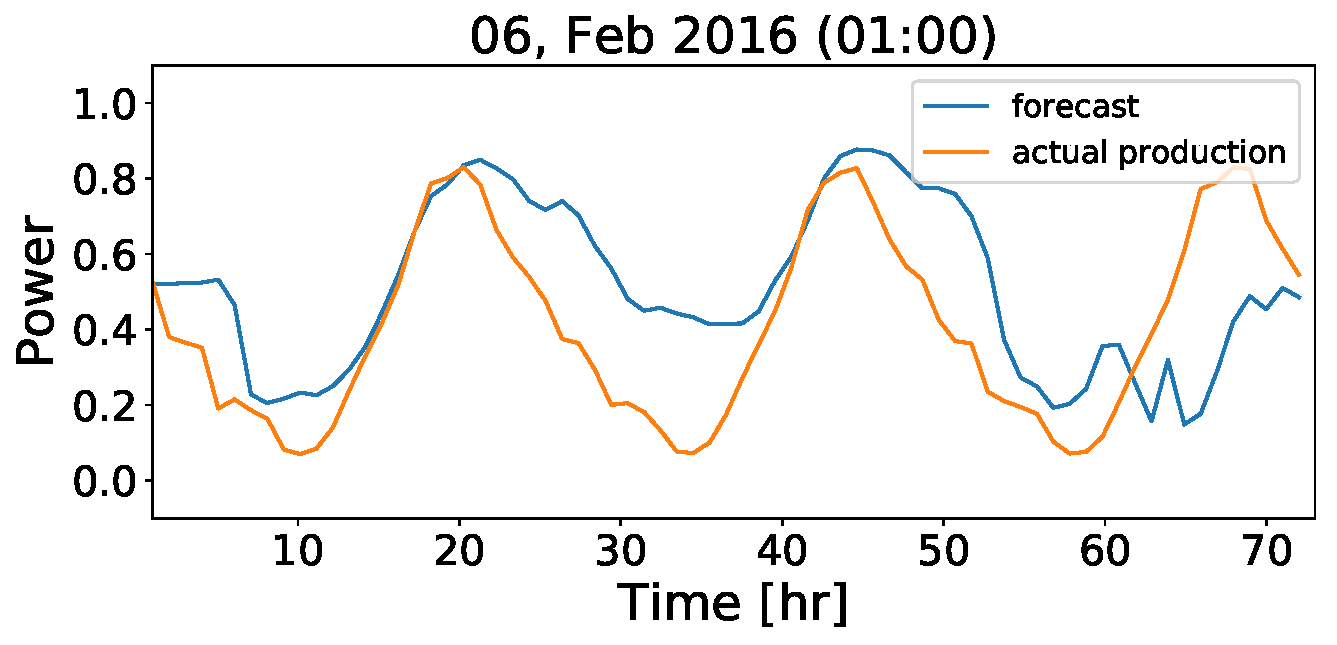
\includegraphics[width=0.8\linewidth]{Forecast_data_68.pdf}
%     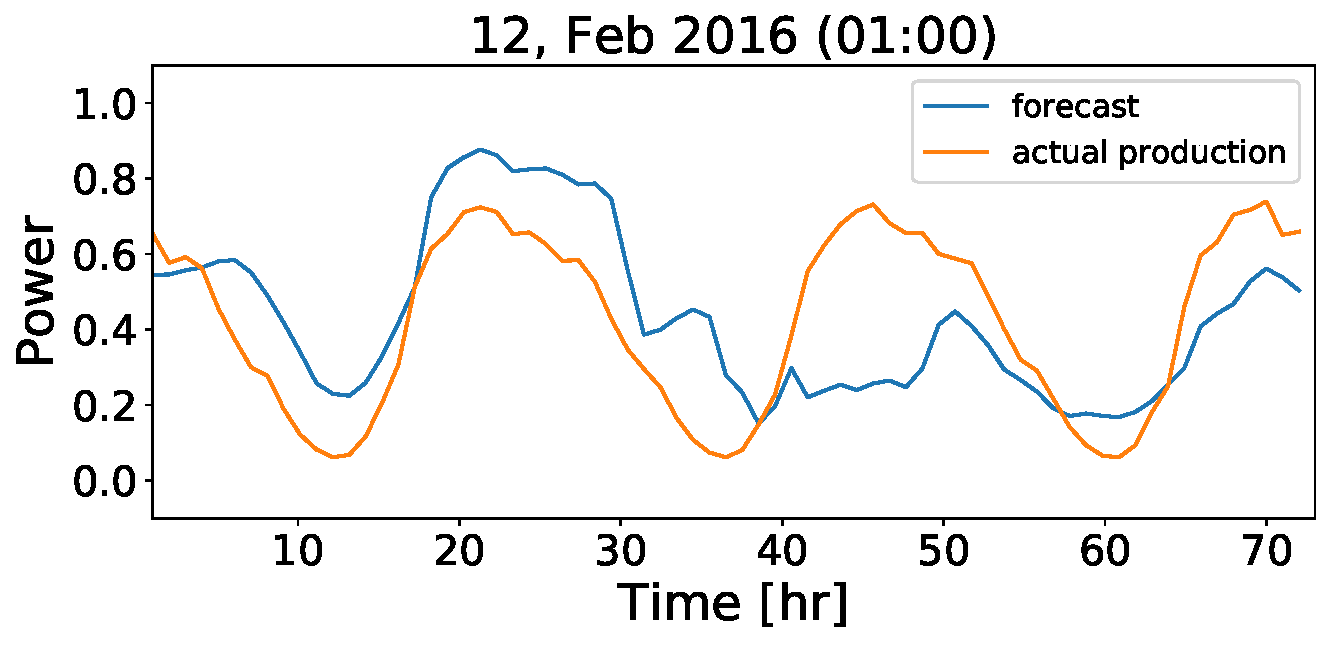
\includegraphics[width=0.8\linewidth]{Forecast_data_82.pdf}
% \end{center}
%    \caption{Examples of wind power generation from the data set along with the wind power generation forecast.}
% \label{fig:long}
% \label{fig:onecol}
% \end{figure}


%%%%%%%%%%%%%%%%%%%%%%%%%%%%%%%%%%%

% \begin{figure}[t]
% \begin{center}
% %\fbox{\rule{0pt}{2in} \rule{0.9\linewidth}{0pt}}
%    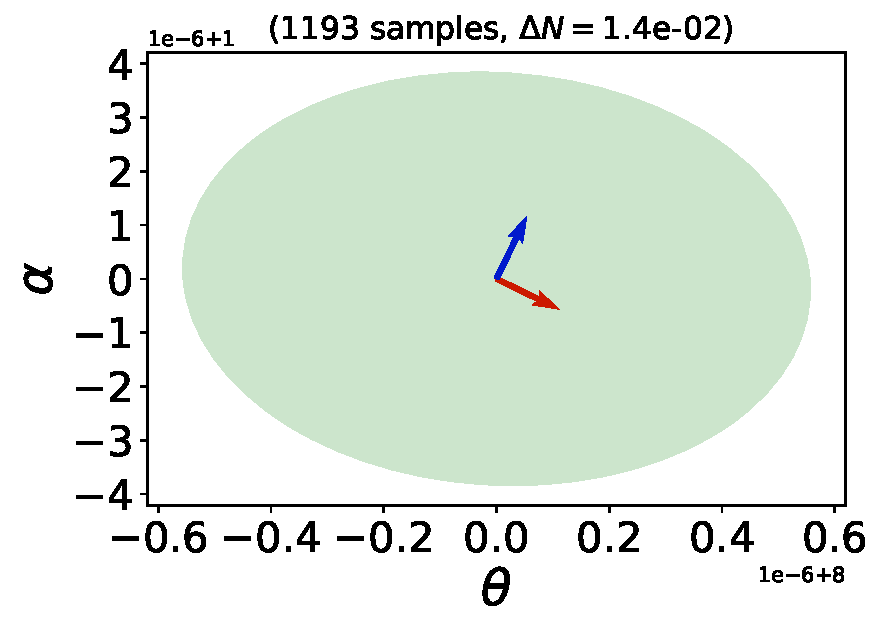
\includegraphics[width=0.6\linewidth]{ellipse1193_samples_dN=14e-02.pdf}
%     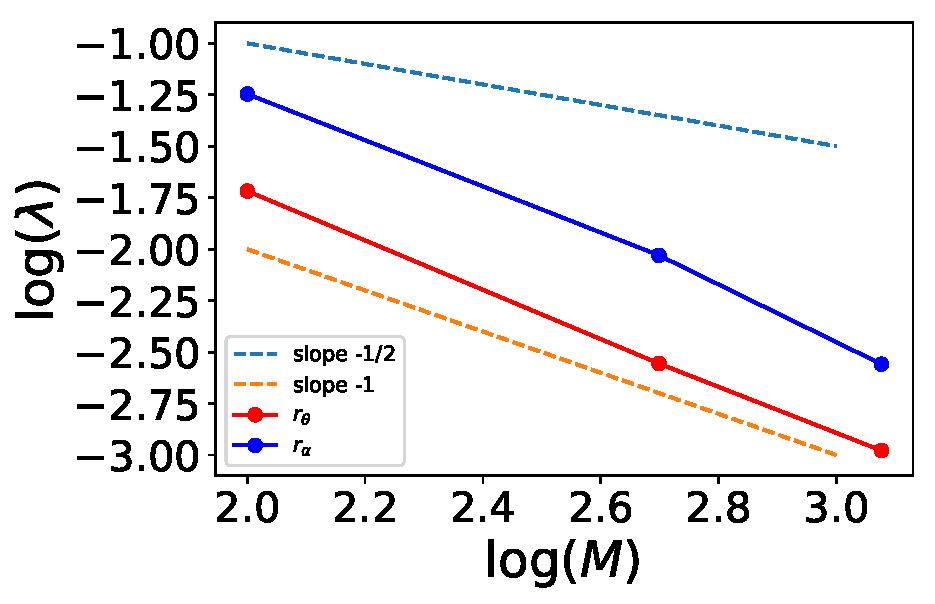
\includegraphics[width=0.6\linewidth]{ellipse_conv_samples_dN=14e-02.pdf}
% \end{center}
%    \caption{Left:Shrinkage of the ellipse determined by the Hessian matrix of the log-likelihood around the point of optimality $(\theta_0^*, \alpha^*)\approx (8,1)$ (Axis are not in natural scale, arrows only to  eignevector direction). Right: Convergence of the major and semi-axis of the ellipse  of the Hessian of the log-likelihood at the point optimality $(\theta_0^*, \alpha^*)\approx (8,1)$. Note that it is slightly faster than the expected rate of $1/\sqrt{M}$. This is due to the correlation structure of the process $V_t$, thus a path may act  as more than one  uncorrelated sample.}
% \label{ellipse_drawing}
% \end{figure}

%  \begin{figure}[t]
% \begin{center}
% %\fbox{\rule{0pt}{2in} \rule{0.9\linewidth}{0pt}}
%    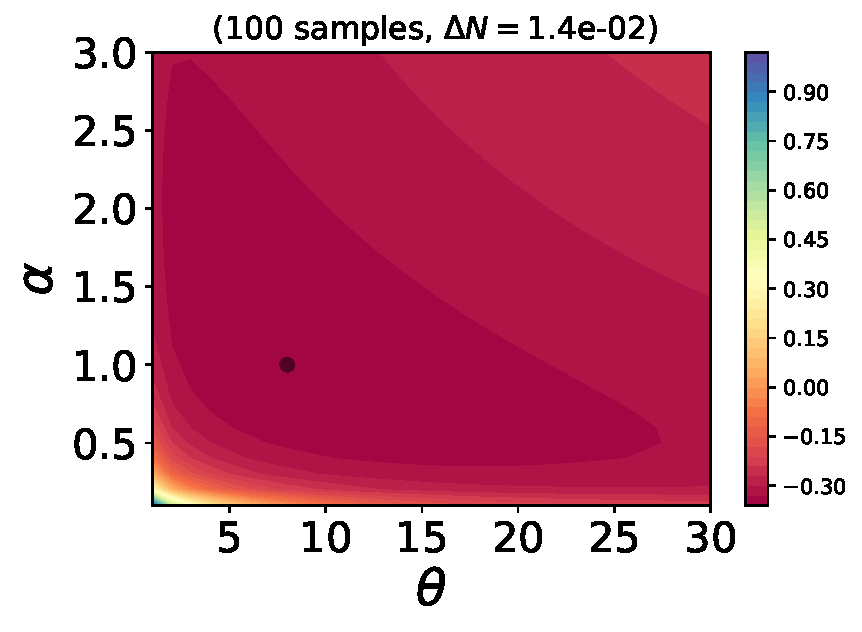
\includegraphics[width=0.9\linewidth]{ISO_100_samples_dN=14e-02.pdf}
%    %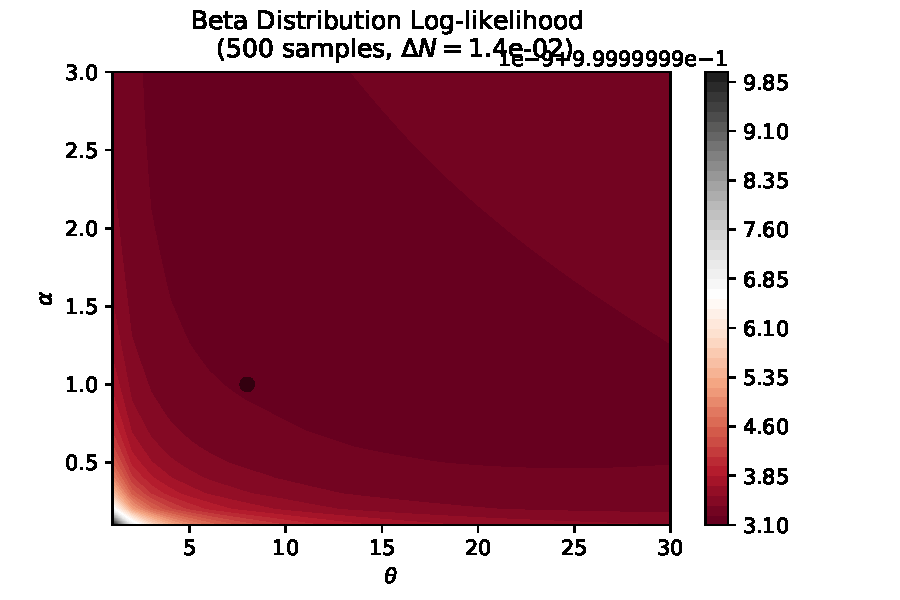
\includegraphics[width=0.5\linewidth]{ISO_500_samples_dN=14e-02.pdf}
%    %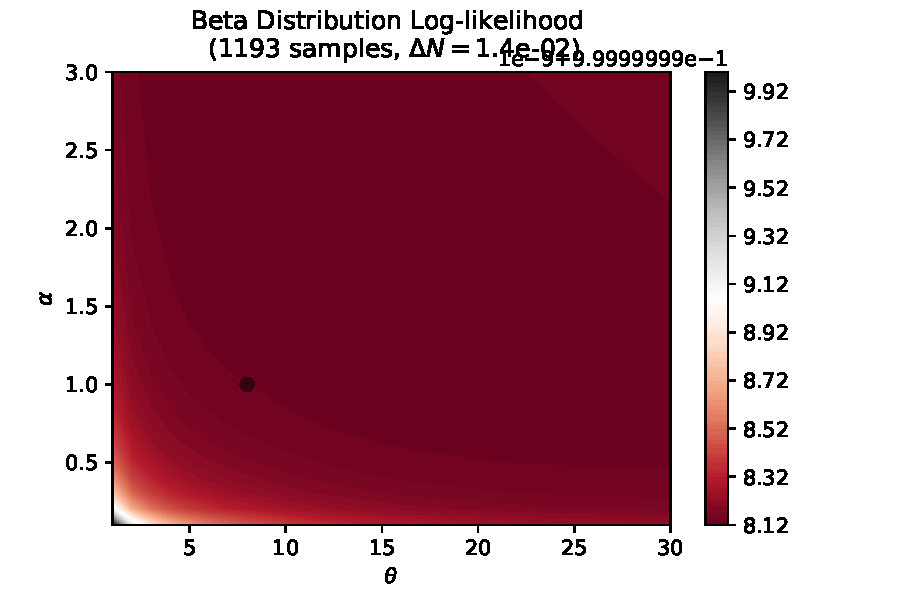
\includegraphics[width=0.5\linewidth]{ISO_1193_samples_dN=14e-02.pdf}
% \end{center}
%    \caption{Contour plot of the log-likelihood with only 100 sample paths, point of optimality $(\theta_0^*, \alpha^*)\approx (8,1)$ indicated by the  black dot.}
% \label{contour}
% \end{figure}


%%%%%%%%%%%%%%%%%%%%%%

% \begin{figure}[t]
% \begin{center}
% %\fbox{\rule{0pt}{2in} \rule{0.9\linewidth}{0pt}}
%    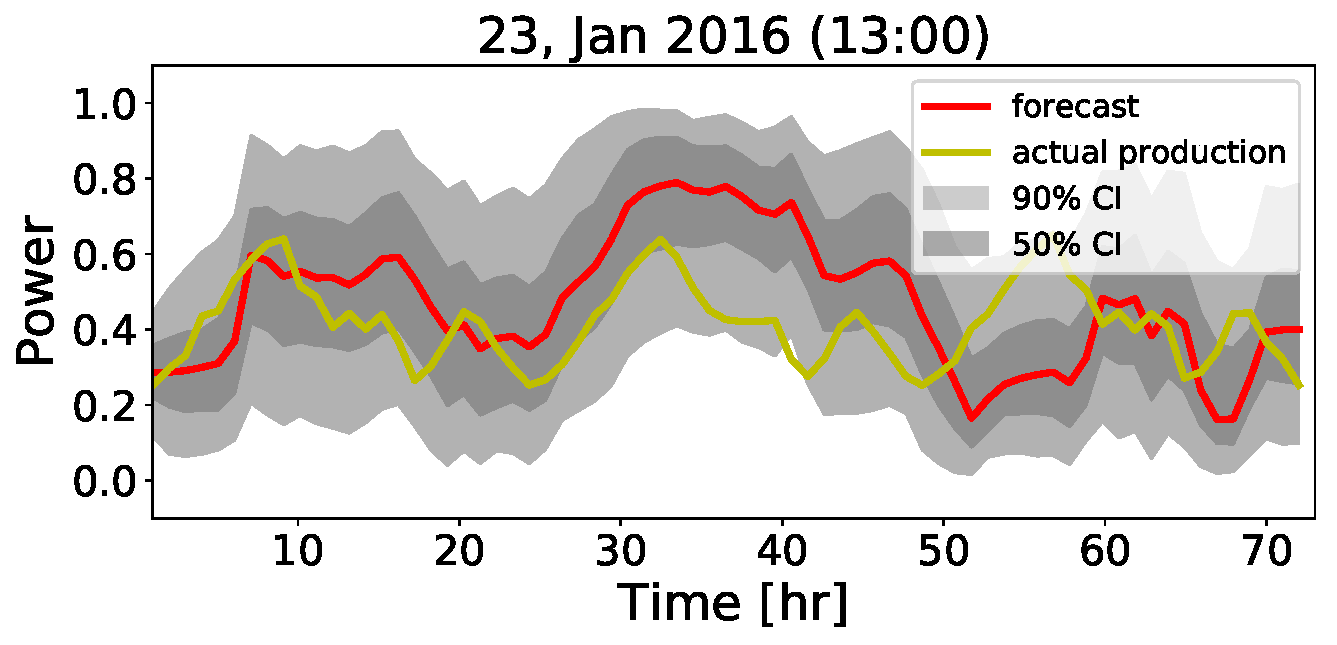
\includegraphics[width=0.8\linewidth]{72hr_forecast_CI_31.pdf} %667
%    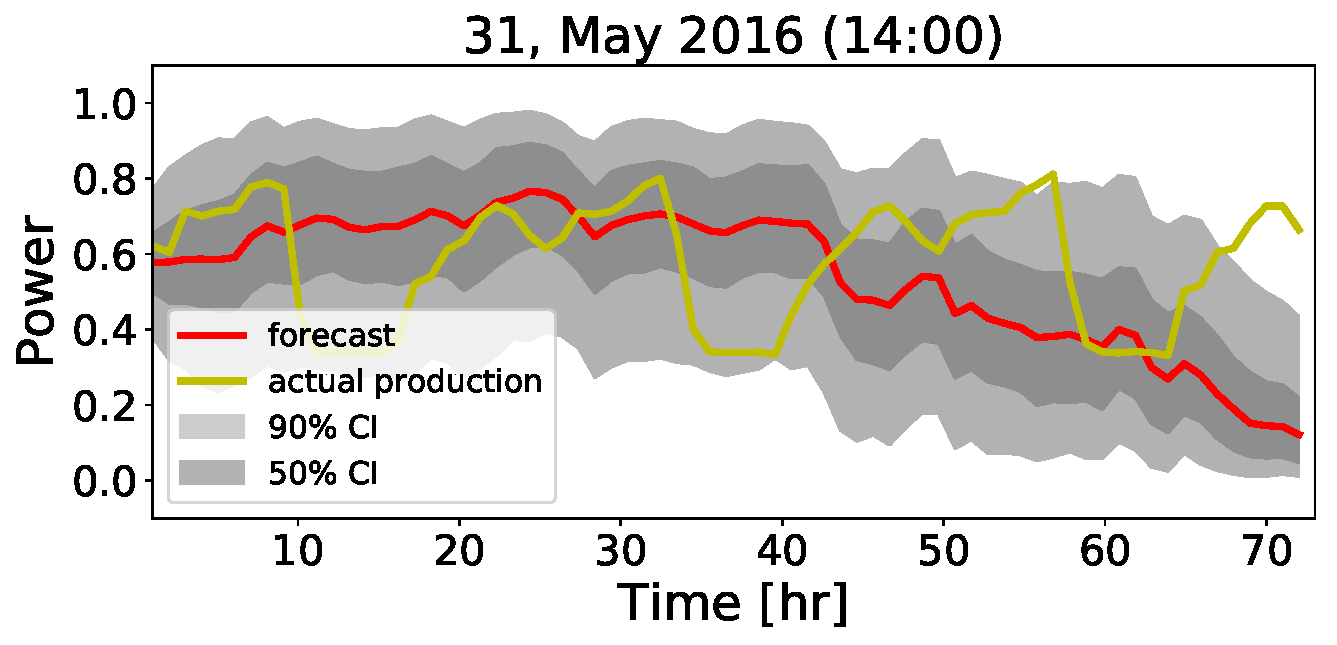
\includegraphics[width=0.8\linewidth]{72hr_forecast_CI_437.pdf}
%    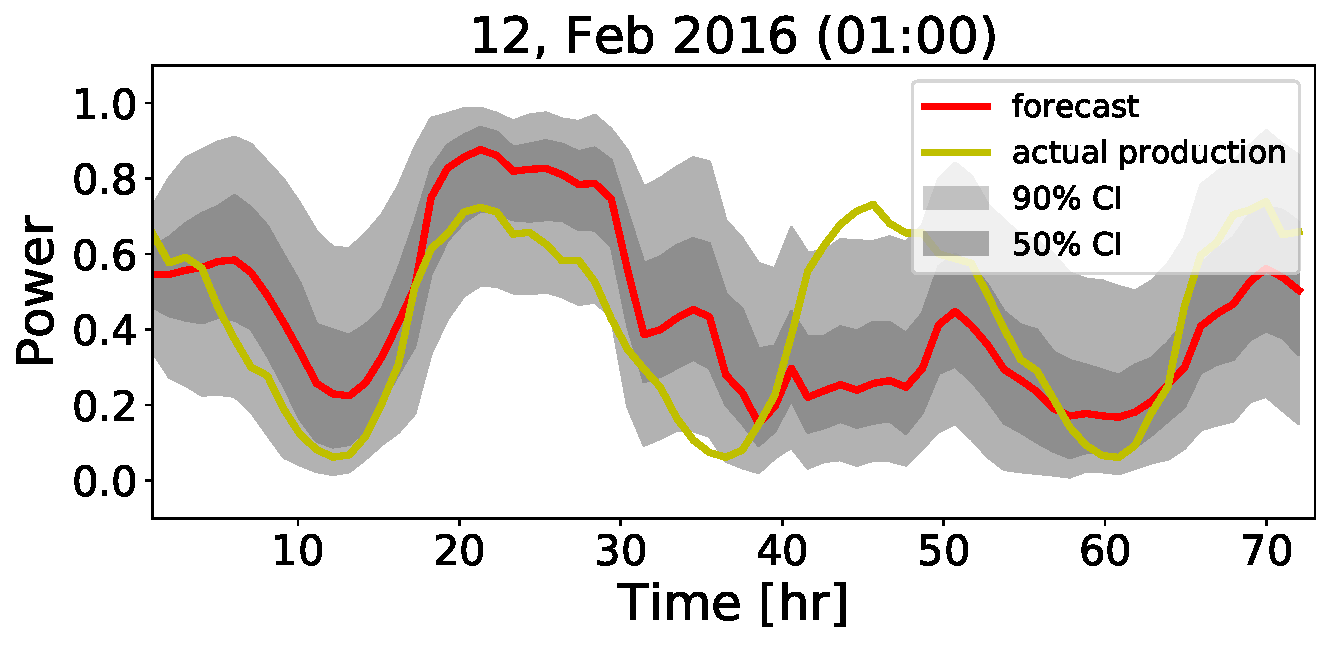
\includegraphics[width=0.8\linewidth]{72hr_forecast_CI_82.pdf}
%
% \end{center}
%    \caption{ Examples of confidence bands obtained for the full 72 hour forecasts.We can see that the model captures the fluctuations in the actual production with non-trivial and asymmetric confidence intervals.}
% \label{fig:72hr}
% \end{figure}
%
% \begin{figure}[t]
% \begin{center}
% %\fbox{\rule{0pt}{2in} \rule{0.9\linewidth}{0pt}}
%    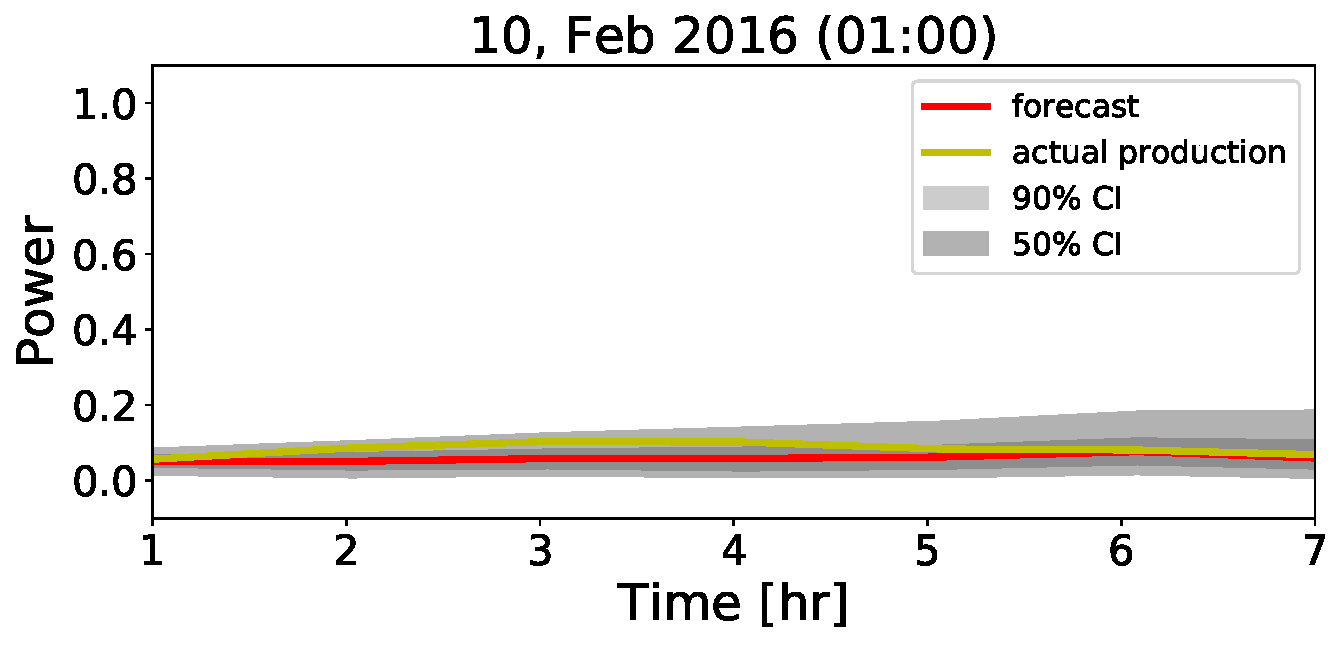
\includegraphics[width=0.8\linewidth]{6hr_forecast_CI_75.pdf}  %569
%    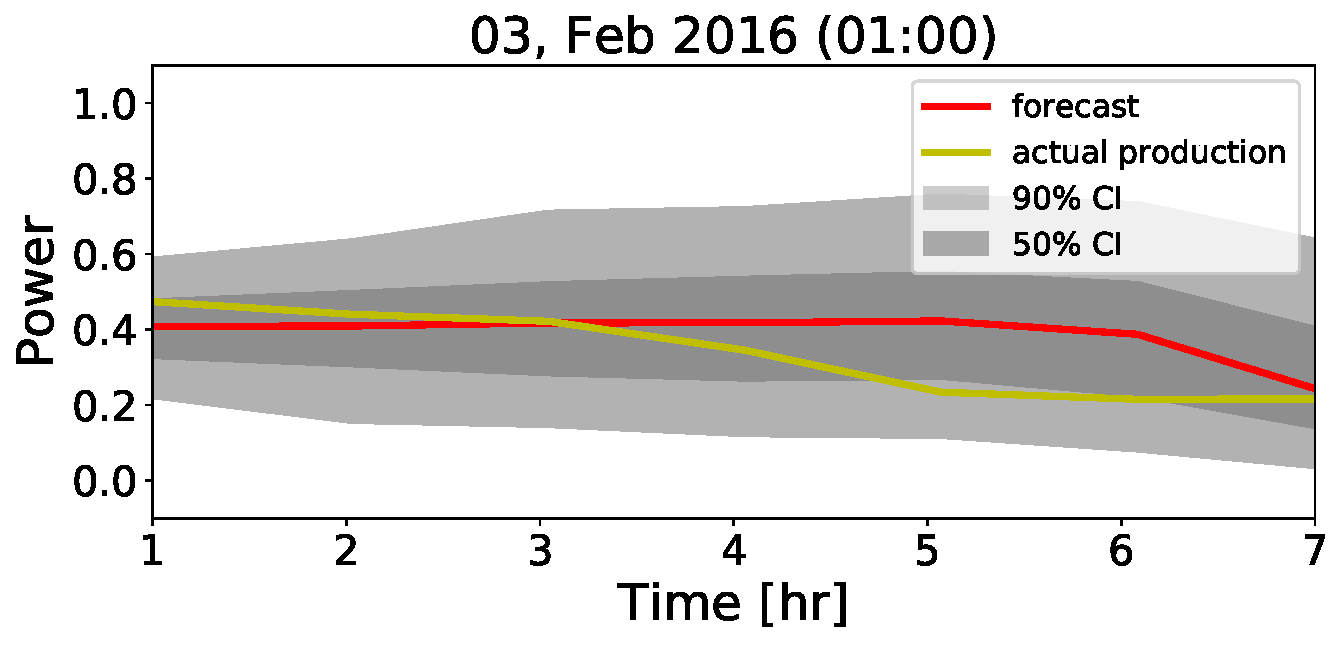
\includegraphics[width=0.8\linewidth]{6hr_forecast_CI_59.pdf}
%    %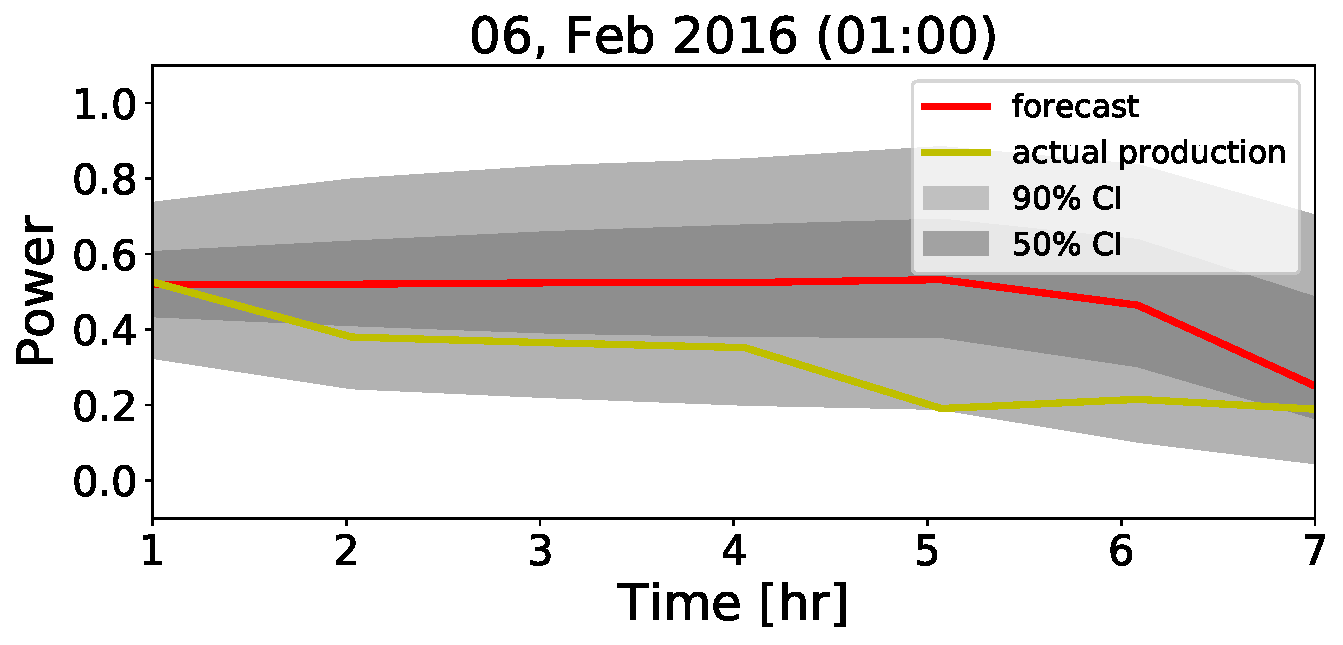
\includegraphics[width=0.9\linewidth]{6hr_forecast_CI_68.pdf}
% \end{center}
%    \caption{ Examples of confidence bands obtained for the first 6 hours of the forecasts. This is important as this specific forecasting company computes a new forecast every 6 hours for reliability.}
% \label{fig:6hr}
% \end{figure}


%  \begin{figure}[t]
% \begin{center}
% %\fbox{\rule{0pt}{2in} \rule{0.9\linewidth}{0pt}}
%    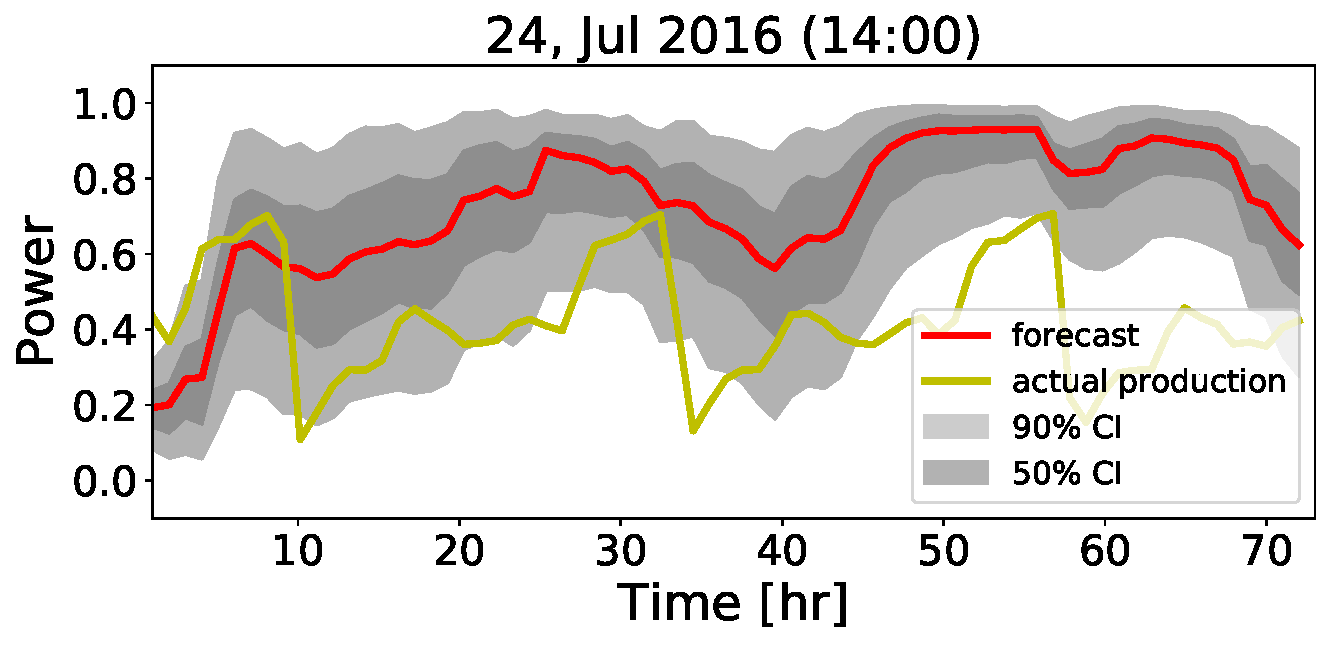
\includegraphics[width=0.8\linewidth]{72hr_forecast_CI_623.pdf}  %569
% \end{center}
%    \caption{ Examples of omitted data which corresponds to production control and manual energy management decisions. In this example,  wind power production was repeatedly curtailed at around 2 AM which is a period of low power demand. Automatic detection of such scenarios is to be incorporated in future works.}
% \label{fig:6hr}
% \end{figure}

%We obtain the modified Beta distribution,
%
%\begin{equation}
%\begin{split}
%f_Y(y; \alpha , \beta )&= f_X(g^{-1}(y) ) \Big| \frac{\partial g^{-1}(y)}{\partial y }  \Big| \\
%&= \frac{1}{B(\alpha, \beta) (b-a)} \Big(\frac{a-y}{b-a}\Big)^{\alpha -1}\Big(1-\frac{a-y}{b-a} \Big)^{\beta -1} \label{modified_Beta}
%\end{split}
%\end{equation}
%where $B(\cdot,\cdot)$ is the Beta function. Also, we have that
%\begin{equation}
%\E[Y]= a + (b-a) \frac{\alpha}{\alpha + \beta}
%\end{equation}
%\begin{equation}
%\V[Y]= (b-a)^2 \frac{\alpha \beta}{(\alpha + \beta)^2 (\alpha + \beta + 1)}
%\end{equation}
